\textbf{``A toda hora e a todo momento''}

Cena 1, Julho de 2005, Oxford, Reino Unido.

Jimmy Wales é convidado ao palco para realizar sua apresentação de 20 minutos no TEDGlobal 2005, primeira edição deste \textit{spin off} das TED Conferences, criado para ``\textit{dar um foco ainda mais forte em ideias realmente grandes para mudar o mundo: memes e sonhos de imbricações de mundos da ciência, arquitetura, tecnologia, negócios e organizações sem fins lucrativos, criatividade global e ingenuidade local}'' \citep{ted_global_2005}.\footnote{No original: ``\textit{even stronger focus on really big world-changing ideas: memes and dreams from the intersecting worlds of science, architecture, technology, business and nonprofit, global creativity and local ingenuity}''.  https://www.ted.com/about/conferences/past-teds/tedglobal-2005 , acessada em 19 de março de 2020.}

A palestra acontece um ano após Wales, ou Jimbo, como é conhecido o fundador mais famoso da Wikipédia dentre seus/suas colegas enciclopedistas, falar em uma entrevista a frase que ele utiliza para abrir a apresentação:\footnote{Palestra disponível em https://www.ted.com/talks/jimmy\_wales\_the\_birth\_of\_wikipedia?language=en , acessada em 19 de março de 2020.}

``\textit{Imagine um mundo onde a toda pessoa do planeta é oferecido acesso livre/gratuito à soma de todo conhecimento humano. É isso que estamos fazendo.}'' \citep{wales_interview_2004}\footnote{Tradução livre. No original: ``\textit{Imagine a world in which every single person on the planet is given free access to the sum of all human knowledge. That's what we're doing.}'' Optamos por traduzir ``\textit{free}" como livre/gratuito pois ambos os sentidos estão presente no uso da palavra neste contexto. }

Em seguida, ele detalha o funcionamento da Wikipédia, explicando que ela é uma enciclopédia em licença livre, feita por milhares de voluntários de todo mundo em vários idiomas, e utiliza um software wiki, um tipo de ferramenta onde \textbf{qualquer um/a pode rapidamente editar}\footnote{ Nesta seção todos os grifos são do autor.} e salvar, com sua alteração indo ao ar para toda a internet imediatamente \citep{wales_birth_2005}.

A apresentação então detalha como a enciclopédia é mantida totalmente por voluntários/as, e que a \textit{Wikimedia Foundation} (WMF), organização sem fins lucrativos criada por Wales para manter a Wikipédia, acabara de contratar seu primeiro e único funcionário em janeiro de 2005, um desenvolvedor de software. É mencionado que o custo de 5 mil dólares com internet é praticamente o único que a organização tem para se manter ativa.

Wales então explica que praticamente não existem controvérsias na escrita de conteúdos na Wikipédia, devido ao fato dos/as editores/as entenderem e respeitarem a política editorial da neutralidade. E conta que as poucas controvérsias que emergem são rapidamente resolvidas, pois não se discutem nem suas verdades  nem suas objetividades, bastando aos/às editores/as relatarem o que os diferentes lados respeitáveis acham da contenda, sem que a enciclopédia precise tomar partido de nenhum deles. A explicação sobre a forma dos/as wikipedistas resolverem controvérsias se encerra com Wales afirmando que esta metodologia funciona pois a comunidade é muito diversa, com membros/as de diferentes origens políticas, religiosas e culturais.

\textbf{Cena 2, Junho de 2015. São Paulo, Brasil.}

Um dos mais de 100 funcionários da WMF participa de uma reunião com voluntários/as interessados/as em criar uma organização no Brasil focada em atividades de extensão do Movimento Wikimedia, nos mesmo moldes de dezenas de outras criadas pelo mundo e financiadas pela WMF, motivados/as pelo fato de que, \textbf{apesar de todos/as poderem editar, poucos/as brasileiros/as editam a Wikipédia}.

Esta é a quarta vez que um grupo tenta criar um ``capítulo Wikimedia''\footnote{No Movimento Wikimedia, capítulos são organizações satélites espalhadas pelo mundo. Esta estrutura será explicada em nosso capítulo 3.} no Brasil, depois das três primeiras fracassarem por atritos, diferenças de visão e impossibilidade de membros da comunidade de trabalharem em conjunto.

Após falar sobre o interesse da Fundação em aumentar a diversidade de seus/suas editores/as, especialmente engajando mais moradores/as do chamado sul global, o funcionário da WMF distribui seu cartão de visitas, onde pode ser lido no verso: ``\textit{Imagine um mundo onde todo ser humano pode compartilhar  livremente/gratuitamente a soma de todo o conhecimento. Este é o nosso compromisso}'' (veja figura \ref{fig:cartao_wmf}).\footnote{Tradução livre. No original ``\textit{Imagine a world in which every single human being can freely share \textbf{in} the sum of all knowledge. That’s our commitment}''. Destacamos o uso do ``\textit{in}'' após o ``\textit{share}'', que passa uma ideia de compartilhamento ativo e por dentro, que é perdida em nossa tradução para o português.}

\begin{figure}[H]
    \centering
    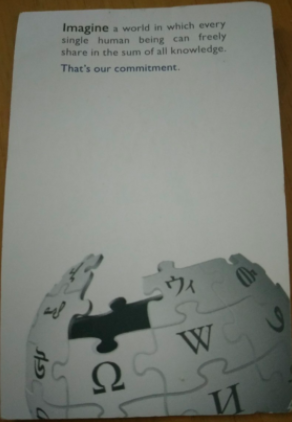
\includegraphics[width=.4\textwidth]{Images/cartao_wmf.png}
    \caption{Verso do cartão de visitas dos funcionários da Wikimedia Foundation.}
    \label{fig:cartao_wmf}
\end{figure}

